\documentclass[./../../paper.tex]{subfiles}
\graphicspath{{\subfix{./../../figures/}}}

\begin{document}
% This section dives into the generative models that we explore in this thesis. They cover fundamentally different approaches to the counterfactual generation of process data. We apply the viability metric established in \autoref{sec:viability} to evaluate the performance of each model.


% Here, we attempt to capture the latent state-space of a model and use this space to sample counterfactual candidates.  Last, we explore a technique which does not require to optimise a differentiable objective function. Instead we use the viability measure as a fitness function and maximise the fitness of each counterfactual candidate.


The generative approach assumes, it is possible to capture a latent state $z$ and use this state to generate suitable counterfactual candidates. We condition the generation procedure on the factual instance to generate counterfactuals that show sparse differences to the original sequence. The core idea is to sample randomly $e^* \sim p(z|e)$ to generate counterfactual candidates. We can sort each candidate by their \emph{viability} and choose top-K contenders as viable couunterfactuals. There are a multitude of approaches to generate the counterfactuals. However, we limit our exploration to a sequential \glspl{VAE}. 
% and sequential \glspl{GAN}. Both technieques allow us to sample from a smooth latent space conditioned on the factual sequence. 
\glspl{VAE} approximate $p(z|e)$ by trying to reconstruct the input using Monte-Carlo methods. For this purpose we encode a sequence into a mean vector. Then we use this vector to reconstruct the initial input again. The architecture resembles the predictor model's architecture, as you can see in \autoref{fig:vae_architecture}.   
% \glspl{GAN} require a generator model and a distriminatior model. The generator model attempts to fool the discriminator model by generating, results that closely resemble true process instances. In contrast, the discriminator tries to distinguish generated instances from real instances.

\begin{figure}[htbp]
    \centering
    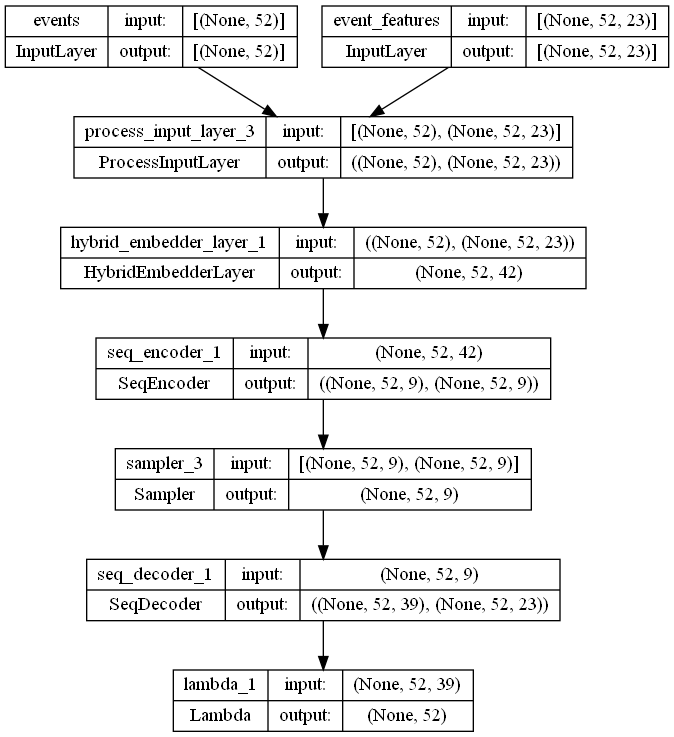
\includegraphics[width=0.8\textwidth]{figures/generator50lstm.png}
    \caption{The different components of the VAE architecture. Each elements contains information about the input and output of a layer. None is a placeholder for the batch size.}
    \label{fig:vae_architecture}
\end{figure}




\end{document}